\section{Technologies}

During the project, we used a variety of technologies to achieve different objectives. For example, we use Docker to manage the whole architecture for the development and the production environments.

\subsection{Docker}

What is Docker? \emph{Docker is an open platform for building, shipping and running distributed applications. It gives programmers, development teams and operations engineers the common toolbox they need to take advantage of the distributed and networked nature of modern applications.}

In iFlux, we prepared several images to instantiate containers on a dedicated VM. Why using Docker? In fact, there are few reasons. Firstly, we can prepare images ready to deploy for other organizations. As the image is self contained, with just few environment variables we are able to instantiate multiple instances of iFLUX easily without having to worry about the deployment itself.

In fact, the iFLUX image, everything is already ready. We have the installation of NodeJS which the runtime that runs our application. All the application dependencies are also bundled as the application is installed. The difference between a dockerized application and a traditional one is that the bundle you ship is self contained and there is nothing to worry about. No more issues with missing dependencies or dependency repository down.

Secondly, it brings a real advantage for the deployment time. As you have your application ready to use and you have just to run one line command to run your containerized application, you have just to download it and to run it. So you can repeat this process on each environment where you want to deploy the app. In our case, we have deployed two distinct productions environments. In summary, we can say prepared once, deploy everywhere.

There is the Docker image file of the iFLUX main server.

\begin{lstlisting}
# Base image which contains node installed
FROM node:0.12.6-wheezy

# Install some dependencies globally to have them in the path
RUN npm install -g grunt bower knex

# Install dependencies with a caching mechanism to improve the Docker image build process
ADD package.json /tmp/package.json
RUN cd /tmp && npm install
RUN mkdir -p /nodejs/iflux && cp -a /tmp/node_modules /nodejs/iflux

# Copy the application in the image
ADD . /nodejs/iflux

# Prepare the user stuff to run the app
RUN useradd -m -r -U iflux \
	&& chown -R iflux:iflux /nodejs/iflux \
	&& chmod +x /nodejs/iflux/start.sh

# Switch the user to let have less privileges than root user
USER iflux

# Set the working directory
WORKDIR /nodejs/iflux

# Expose the application port
EXPOSE 3000

# This instruction will be used when the container will instantiated
CMD ./start.sh
\end{lstlisting}

The script that will be run once the container is instantiated is the following.

\begin{lstlisting}
#!/bin/bash

# Run the database migration. Ensure that the database is ready each time the application is updated and redeployed
knex migrate:latest

# Start the application. Remember we are in the working directory where the application is deployed.
npm start
\end{lstlisting}

\subsubsection{Docker Compose}

We did the work to create the images for each component of iFLUX. For the database, the different action targets and event sources. Pretty much everything is dockerized. Therefore, we need an orchestration tool to manage all the containers. For that, Docker is shipped with a tool called Docker Compose. This tool allow us to prepare a configuration. The configuration contains the definition of each service and their dependencies. With that, Docker Compose is able to calculate the start order regarding the dependency graph. For example, Docker Compose will start the database used by iFLUX before the server will start.

\label{lst:docker-compose-conf}
\begin{lstlisting}
# The API documentation is exposed through static website on port 4000
ifluxapidoc:
  image: softengheigvd/iflux-apidoc:latest
  env_file: ./.env
  ports:
    - "4000:4000"

# This is a container to handle the data of all the service. In real production use case, each service will have its own data container. With this configuration, the storage is stored on the host running Docker containers and then will ensure the data are persisted between to run of a container.
ifluxsrvdata:
  build: iflux-server-data
  volumes:
    - "/iflux/db/mongo:/data/db"
    - "/iflux/db/postgres:/var/lib/postgresql/data"
    - "/iflux/kafka:/kafka"
    - "/iflux/esearch:/usr/share/elasticsearch/data"
    - "/iflux/slack:/data/slack"
    - "/iflux/viewbox:/data/viewbox"
    - "/iflux/metrics:/data/metrics"
    - "/iflux/publibike:/data/publibike"
    - "/iflux/citizen:/data/citizen"

# The main service of iFLUX. This piece contains the logic to evaluate the rules.
ifluxsrv:
  image: softengheigvd/iflux-server-node:latest
  env_file: ./.env
  ports:
    - 3006:3000
  links:
    - postgresql
    - kafka
    - zookeeper:zk
    - elasticsearch:es

# This component receive the events before forwarding them to Kafka to let iFLUX main component to consume the events.
ifluxapi:
  image: softengheigvd/iflux-api-gateway-node:latest
  env_file: ./.env
  ports:
    - 3005:3000
  links:
    - ifluxsrv
    - kafka
    - zookeeper:zk

# The frontend to manage the iFLUX data (configuration, ...)
ifluxfe:
  image: softengheigvd/iflux-frontend
  env_file: ./.env
  ports:
    - 3007:3000

# This is an action target to send Slack messages
ifluxslack:
  image: softengheigvd/iflux-slack-gateway:latest
  env_file: ./.env
  ports:
    - 3001:3000
  volumes_from:
    - ifluxsrvdata

# Another action target to collect and manage metric collections
ifluxmetrics:
  image: softengheigvd/iflux-metrics-action-target:latest
  env_file: ./.env
  links:
    - mongo
  ports:
    - 3002:3000
  volumes_from:
    - ifluxsrvdata

# One more action target to visualize geolocalized data
ifluxmapbox:
  image: softengheigvd/iflux-mapbox-viewer:latest
  env_file: ./.env
  ports:
    - 3004:3000
  volumes_from:
    - ifluxsrvdata

# This action target is prototype realized in the context of Paleo Festival to show the parking in/out activity.
ifluxpaleo:
  image: softengheigvd/iflux-paleo-2015:latest
  env_file: ./.env
  links:
    - mongo
  ports:
    - 3008:3000
  volumes_from:
    - ifluxsrvdata

# This component is a bit special as it serves to populate the data for a first deployment of iFLUX. It interacts directly with the iFLUX APIs.
ifluxstarter:
  image: softengheigvd/iflux-server-starter:latest
  env_file: ./.env

# This event source was originally a project in a course at the school. We took the opportunity to integrate iFLUX to send events.
citizen:
  image: softengheigvd/citizen:latest
  env_file: ./.env
  links:
    - mongo
  ports:
    - 3003:3000
  volumes_from:
    - ifluxsrvdata

# This component is a poller of the publibike service which will emit events with the state of the different bike stations.
publibike:
  image: softengheigvd/iflux-publibike-event-source:latest
  env_file: ./.env

# Mongo is used by the metrics component as backend to store the data.
mongo:
  image: mongo
  command: mongod --smallfiles
  ports:
    - 27017:27017
  volumes_from:
    - ifluxsrvdata

# Postgresql is used to store the data of iFLUX. Data in this context are all the entities that allow configuring and managing the rules.
postgresql:
  image: postgres:9.4
  volumes_from:
    - ifluxsrvdata
  volumes:
    - "./db:/docker-entrypoint-initdb.d"
  ports:
    - 5432:5432
  env_file: ./.env

# This tricky component is just a timer to let postgresql finishing to initialize itself.
postgresqlwait:
  image: n3llyb0y/wait
  links:
    - postgresql:db
  environment:
    PORTS: 5432

# Zookeeper comes with Kafka. This let kafka working well.
zookeeper:
  image: wurstmeister/zookeeper
  ports:
    - 2181:2181

# Kafka is the messaging bus used between iFLUX API Gateway and iFLUX
kafka:
  image: wurstmeister/kafka
  ports:
    - 9092:9092
  links:
    - zookeeper:zk
  environment:
    KAFKA_CREATE_TOPICS: "iflux-events:1:1"
  env_file: ./.env
  volumes_from:
    - ifluxsrvdata
  volumes:
    - /var/run/docker.sock:/var/run/docker.sock

# Elastic search is used to store the events and rules evaluation results for later analysis and querying
elasticsearch:
  image: elasticsearch:1.5.2
  volumes_from:
    - ifluxsrvdata
  ports:
    - 9200:9200
    - 9300:9300

# Kibana is a web user interface to interact with ElasticSearch
kibana:
  image: shortishly/kibana
  links:
    - elasticsearch
  ports:
    - 5601:5601

# This component is not mandatory but in our case and due to technical limitations we have in the infra where iFLUX is hosted, we put in place a reverse proxy that is exposed to another one. Acting like this allow us managing our different components in any way we want but remaining stable for the front reverse proxy.
rp:
  build: rp
  links:
    - kibana
    - ifluxpaleo:paleo
    - ifluxmapbox:viewbox
    - ifluxmetrics:metrics
    - ifluxslack:slack
    - ifluxapi:gateway
    - ifluxsrv:iflux
    - ifluxfe:fe
    - ifluxapidoc:doc
    - citizen
    - publibike
  ports:
    - 3000:80
\end{lstlisting}

In fact, it's not enough to run the complete service with peace. We discovered that Docker Compose will not wait that a started service is ready. What does it mean? Starting a database requires time, especially when nothing is initialized. When you start such service, the foreground process managed by Docker is ready but the service itself is not. As Docker consider the container running and then the service running, it will continue with the next steps in its launch order. But sometimes, your service is really not ready when the service that depends on it tries to access it and fails.

For that, we discovered some useful images that allow us to make a kind to timer which will wait until the real service and not just the process is ready. Therefore, we have bundle all that stuff in a running script that we use to start the whole infrastructure.

\begin{lstlisting}
#!/bin/bash

docker-compose run --rm postgresqlwait

docker-compose up -d rp

docker ps
\end{lstlisting}

\subsubsection{Docker Hub}

In addition, we use \emph{Docker Hub} which is a platform offered by the creators of Docker to upload/download images. Once they are published on their platform, they are available to everybody. As iFLUX is an Open Source project, we decided to publish the corresponding images to the community. Moreover, we have also facilitated the deployment process on the school server where we have just to download the latest versions of the images. This also confirmed the goal of Docker which can be summarized as: \emph{Build once, deploy everywhere}.

\subsection{Kafka}

What is Kafka? \emph{Apache Kafka is publish-subscribe messaging rethought as a distributed commit log.} The Kafka website is saying the following:

\begin{itemize}
\item\textbf{Fast}: A single Kafka broker can handle hundreds of megabytes of reads and writes per second from thousands of clients.
\item\textbf{Scalable}: Kafka is designed to allow a single cluster to serve as the central data backbone for a large organization. It can be elastically and transparently expanded without downtime. Data streams are partitioned and spread over a cluster of machines to allow data streams larger than the capability of any single machine and to allow clusters of co-ordinated consumers
\item\textbf{Durable}: Messages are persisted on disk and replicated within the cluster to prevent data loss. Each broker can handle terabytes of messages without performance impact.
\item\textbf{Distributed by Design}: Kafka has a modern cluster-centric design that offers strong durability and fault-tolerance guarantees. 
\end{itemize}

Kafka is designed to be highly scalable. Then it is usually used in a cluster mode of multiple instances of Kafka. Zookeeper is used to orchestrate the Kafka cluster. Even if you only used one Kafka instance, Zookeeper is required to store topic and partitions metadata.

Kafka comes with several concepts:

\begin{itemize}
\item\textbf{Consumer} is the part that will get the messages from the topics. The consumer keep the state of which message has to be read or not. It maintains which is called an offset of the partition it is interacting with. In fact, the offset is free of manipulation meaning you can read old messages at anytime as long as they remains in the topic (timeout limit to free space);
\item\textbf{Producer} is the part that will creates and sends the message to Kafka;
\item\textbf{Topic} is the way to organize the messages;
\item\textbf{Partition} is inside a topic. This will allow to scale a topic in the Kafka cluster. You can have one topic with several partitions. The Producer and Consumer can interact, in a round robin way for example, with specific partitions. The messages that arrives in a partition are guaranteed to be stored in the received order.
\end{itemize}

In iFLUX, we use Kafka for the messaging between the API gateway and the rule engine. So the API gateway is our producer and the iFLUX rule engine is our consumer. We defined one topic to exchange the messages.

One of the advantage of Kafka is the availability of a lot of clients in different languages. We found, at least, one for NodeJS and then we were able to integrate Kafka in our two components.

The code to achieve that is pretty straight forward. For the producer part, it requires to create and connect a client and then to create a producer. Once the producer is ready, we can post messages to the topic we want. Kafka can auto-create the topic if missing.

\begin{lstlisting}
var client = kafka.Client('<zookeeperhost:zookeeperport>', 'clientId');
var producer = new Producer(client);

// Error handling, there just print to the console the error message
producer.on('error', function(error) {
	console.log(error.message);
});

// Example of message sent to a topic. In fact, two messages are sent at the same time.
producer.send([{ 
	topic: 'topicName', 
	messages: [{
		content: "First message"
	}, {
		content: "Second message"
	}]
]}, function(err, data) {
	// Function to handle any error during the messages are sent
	if (err) {
		console.log(err.message);
	}
});
\end{lstlisting}

The code for the consumer is a little bit more tricky. This is due to the fact we have to manage the deconnection/reconnections.

\begin{lstlisting}
var client, consumer, producer;

// This function will handle the message when they arrive. This is the entry point that 
// will trigger the rule evaluation for each message received. In iFLUX, each message 
// corresponds to one event.
function messageHandler(message) {
	var time = timeService.timestamp();
	var events = JSON.parse(message.value);

	// A message can be an array of events depending if the gateway 
	// received one event or multiple events
	if (!_.isArray(events)) { events = [ events ]; }

	// Code to save the events in ElasticSearch is removed for readability
	...

	// Trigger the rule evaluation
	ruleEngineService.match(events);
}

// In case of error, we will handle it and set a timeout before trying to
// reconnect to the broker
function consumerErrorHandler(error) {
	if (!_.isUndefined(error)) { console.log(error); }

	// Setup timeout to wait before trying to reconnect to Kafka
	setTimeout(setup, 5000);
}

// Do the configuration against Kafka. Establish the consumer 
// connection with the previous offset if known.
function consumerSetup(offset) {
	consumer = new Consumer(
		client, 
		[{ topic: 'topicName', offset: offset }], 
		{ fromOffset: true }
	);

	// Setup the handlers on the consumer
  	consumer.on('message', messageHandler);
	consumer.on('error', consumerErrorHandler);
}

// Retrieve the last offset in case of failures and the current client state is lost.
// This strategy avoid re-consuming messages already handled.
function offsetSetup() {
	// Create the offset object
	var offset = new Offset(client);

	// Once the offset is ready, retrieve the value for the topic
	offset.on('ready', function() {
		offset.fetch([{ topic: 'topicName', time: -1 }], function (err, data) {
			consumerSetup(data['topicName'][0][0]);
		});
	});
}

// General setup at the application startup or when the connection to Kafka is lost
function setup() {
	// Close the client if necessary
	if (client) {
		try { client.close(); }
		catch (err) { console.log(err); }
	}

	// Close the consumer if necessary
	if (consumer) {
		try { consumer.close(); }
		catch (err) { console.log(err); }
	}

	// Connect to Kafka through Zookeeper (handled by the NodeJS module)
	client = kafka.Client('<zookeeperhost:zookeeperport>', 'clientId');

	// Setup the offset
	offsetSetup();
}

// At application startup, we call the main setup operation
setup();
\end{lstlisting}

With these two code parts respectively in iFLUX API Gateway and iFLUX core server, we are able to send and receive event through Kafka messages. One of the advantage is the possibility to do some maintenance. We can stop iFLUX core server without loosing any message. In fact, the API gateway will continue to receive the message and to post them into Kafka. Kafka will store the messages for a certain period of time in the order that the messages arrived. Then, once the iFLUX core server is up again, he consume all the messages not already consumed.

Another use case where Kafka is really useful is when we encounter a high traffic of events. We can add more API Gateway nodes in our infrastructure to absorb the high traffic. All the messages will be handled by the Kafka cluster (at condition we have setup a correct Kafka infrastructure with sufficient nodes, RAM and storage). The rule engin on the iFLUX core can therefore take the time to handle the messages. This approach will surely differ the message evaluation but at least, no event will be lost or not evaluated.

\subsection{ElasticSearch}

What is ElasticSearch? \emph{Elasticsearch is a distributed, open source search and analytics engine, designed for horizontal scalability, reliability, and easy management. It combines the speed of search with the power of analytics via a sophisticated, developer-friendly query language covering structured, unstructured, and time-series data.}

We use ElasticSearch to archive the events received in the iFLUX core server before the rules evaluation. We keep an unmodified version of the event. Once, the rules are evaluated, we also keep the result of the evaluation and what matched in the rule regarding the event. Therefore, we have two different indexes in ElasticSearch where we can perform text search queries.

With the addition of Kibana, we have a frontend dedicated to ElasticSearch where we can build personal dashboards to make the data more useful. The different graphs can be created based on ElasticSearch queries defined by the users.

In this project, we also used ElasticSearch and Kibana as debug tools to get more logs on when and where things are happening. It helps to answer questions like: Is my event evaluated positively by this rule? Is my event received by the iFLUX core server? And so on.

In addition, keeping the events in ElasticSearch let us the possibility to do post processing on the data collected. If we have missed a possibility to add value on the data by doing a specific processing, we have the possibility to extract those data from ElasticSearch as long as we keep the data. In our setup, we have not set any purge mechanism and keep the data for lifetime.

The integration of ElasticSearch in NodeJS application is also simple like we have done for Kafka. There is an example of integration below.

\begin{lstlisting}
// Setup the client to connect to ElasticSearch
var client = new elasticsearch.Client({
	host: '<elasticSearchHost>:<elasticSearchPort>',
	log: 'info'
});

// Create the payload to save in ElasticSearch 
// and the related configuration
var esItem = {
	index: 'indexName',
	type: 'json',

	// We use a UID generator to have unique ID
	id: 'randomUniqueId', 
	body: {
		// Take care that the ID fields cannot be named id
		_id: "a business id not related to ES', 

		// ElasticSearch works better with dates in data
		timestamp: new Date() 

		content: "A user defined content",
	}
};

// Create the ElasticSearch entry
client.create(esItem, function (error, response) {
	// Error handling
	if (!_.isUndefined(error)) {
		console.log(error);
		console.log(response);
	}
	else {
		console.log('Model persisted in ElasticSearch');
	}
});
\end{lstlisting}

By the way, our system is fault tolerant with ElasticSearch. If ElasticSearch is not available, it will not block or cause any issue in the rules evaluation or event reception. 

\subsection{Storm}

What is Storm? \emph{Apache Storm is a free and open source distributed real time computation system. Storm makes it easy to reliably process unbounded streams of data, doing for real time processing what Hadoop did for batch processing. Storm is simple, can be used with any programming language, and is a lot of fun to use!}

Storm comes with several concepts:
\begin{itemize}
\item\textbf{Topology} is a graph more exactly a Directed Acyclic Graph, of spouts and bolts that are connected with stream groupings. 
\item\textbf{Spout} is a source of streams in a topology. One of the most common source is Kafka. 
\item\textbf{Bolt} is a processing unit used to filter, aggregate, join, talk to database, custom function, etc. It is the logical function inside Storm. 
\item\textbf{Streams} is the core abstraction in Storm and more precisely a sequence of tuples. 
\item\textbf{Worker} is a physical JVM that contains executors. 
\item\textbf{Executors} is a worker thread that executes one or many tasks.
\item\textbf{Tasks} is a bolt or spout to process.
\item\textbf{Nimbus} is a daemon running on the master node. It distributes the code on the cluster, assign task to supervisors and watch errors. 
\item\textbf{Supervisor} is a daemon running on slaves nodes. They receive jobs assigned to these workers. For each worker there is one supervisor daemon. 
\end{itemize}


Storm guarantees that every spout tuples will be fully processed by the topology. A spout is considered as fully processed when the tree of tuples has been successfully completed. If a worker is down or a task make more than X seconds (Timeout defined by the user) to process, the tree tuples is considered as failed, and the spout send again the data. One master node check the availability of each worker and if one is down, it restart it or redeploy a new one in another location in the cluster. 

The purpose of using Storm in iFlux is to be scalable with the amount of events to process. A good start will be to modify the iFlux server which evaluate the rules by encapsulating it in a Bolt. The figure \ref{fig:iflux-storm-architecture} explains the architecture. 

\begin{figure}
\centering
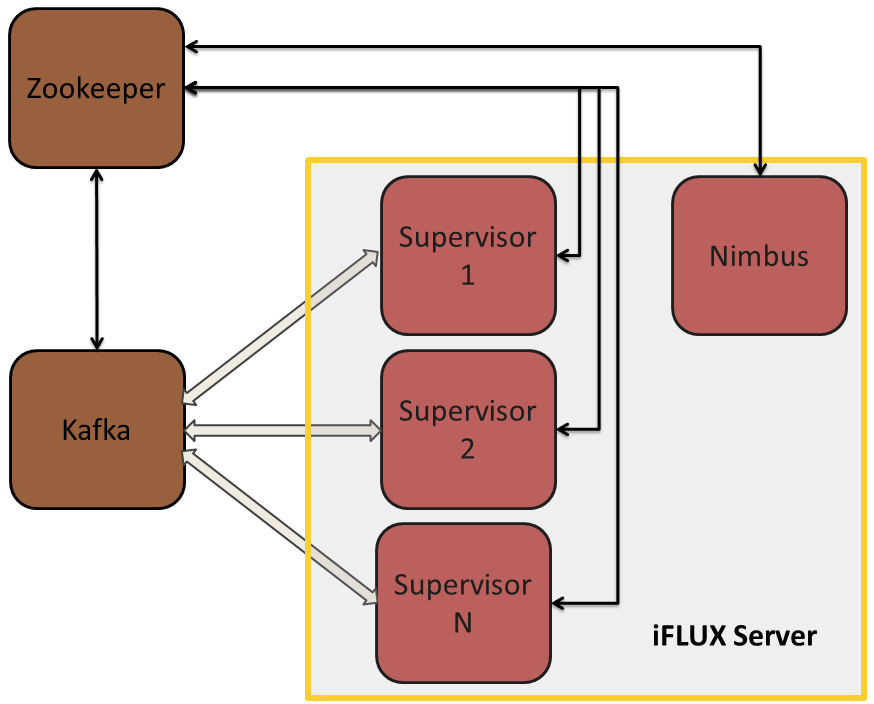
\includegraphics[width=1\columnwidth]{figures/storm-architecture.png}
\caption{Storm architecture concept}
\label{fig:iflux-storm-architecture}
\end{figure}

Each box is a docker container and by definition can be deployed on a physical server. Storm is built to run JVM languages as bolt, but it also provide a Multilang protocol to support other language. Multilang use json messages over stdin/stdout to communicate with the subprocess. The topology will have one Spout which reads events from Kafka and push them to the Bolt thats evaluate the rules. The bolt is parallelized as you want and make the architecture scalable and fault tolerant. The figure \ref{fig:iflux-topology} 
displays the topology with Kafka interactions and the result Actions. 

 \begin{figure}
\centering
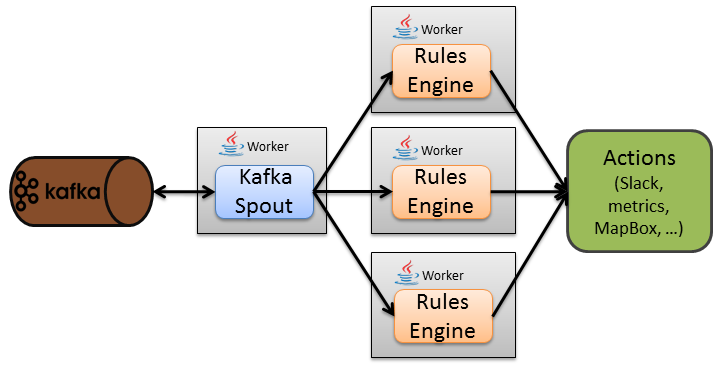
\includegraphics[width=1\columnwidth]{figures/storm-topology.png}
\caption{Storm topology with bolt in parallel}
\label{fig:iflux-topology}
\end{figure}

A better architecture will be to undockerize Kafka, Zookeeper and Storm and run them in native environment to enhance performances. The second optimization is to decompose the rules engine in small tasks and create an acyclic graph which is a Storm topology. The goal is to avoid the unique bolt and replace it by a real Storm topology with many bolts. All infrastructure can be deployed on a Hadoop cluster. 

\subsection{API Testing}

During the development of iFLUX core API, we have updated so many times the API that it started quickly to be a nightmare to do not introduce any regression. We decided to implement a full test coverage at the API level. We have investigated several solutions to write our API tests in NodeJS but we did not find any suitable solution that will allow to write long scenario (ex: Create a resource, update this resource, list all the resource to see if this one is included, delete this resource). And no solution permit to avoid the Pyramid of Doom problem of NodeJS callbacks.

We finally reach the point to use a tool called API Copilot which is wrapper around a node module to write REST requests. This tool allow to write scenario in the purpose to populate a service which offer a REST Service. It largely use promises as a core concept to avoid the pyramid. So, from a code like that

\begin{lstlisting}
// First call
client.get('/users', function(result) {
	// ... do something with result

	// Second call
	client.get('/rules', function(secondResult) {
		// ... do something with secondResult

		// Third call
		client.get('/actionTargets', function(thirdResult) {
			// ... do something with thirdResult
			... and so on with more indentations and callbacks
		});
	});
});
\end{lstlisting}

we achieve to have a cleaner code

\begin{lstlisting}
client
	// First call
	.get(function(result) {
		// ... do something with result
	})
	
	// Second call
	.get(function(result) {
		// ... do something with result
	})
	
	// Third call
	.get(function(result) {
		// ... do something with result
	})
;	
\end{lstlisting}

So, with API Copilot, we have the proper tool to do REST API calls in order and to do some processing with the responses to react for the next steps. What we did is just a wrapper to be able to dynamically add new steps. We also added some assertions and logging. There is an example of a test suite.

\begin{lstlisting}
// Create the test suite
var testSuite = new TestSuite('Authentication resource')
	// Configure the base URL for all the following calls
	.baseUrl('http://localhost:3000')
	
	// Set the Content-Type header to be application/json
	.setJson();

// Define a test
testSuite
	// Give a description to the test
	.describe('Unknown user cannot signin')
	// Do a POST request with a content body
	.post({
		url: '/v1/auth/signin',
		body: {
			email: 'henri.dupont@localhost.localdomain',
			password: 'password'
		}
	})
	// Assert the response code
	.expectStatusCode(401);

// Second test that will be run after the first one
testSuite
	.describe('Register new user')
	.post	({
		url: '/v1/auth/register',
		body: {
			email: 'henri.dupont@localhost.localdomain',
			firstName: 'Henri',
			lastName: 'Dupont',
			password: 'password',
			passwordConfirmation: 'password'
		}
	})
	.expectStatusCode(201)
	// Assert the location header is present and is correct
	.expectLocationHeader('/v1/me');

// Third test that will be run after the second one. This one depends
// on the previous one. So in the second test we created the user
// and in this test we try to sign-in with the just created user.
testSuite
	.describe('Valid authentication')
	.post({
		url: '/v1/auth/signin',
		body: {
			email: 'henri.dupont@localhost.localdomain',
			password: 'password'
		}
	})
	.expectStatusCode(200)
	// Assert the JSON content received contains a 
	// field token at the first level.
	.expectJsonToHavePath('token');

// Export the test suite to let the wrapper to execute the tests
module.exports = testSuite;
\end{lstlisting}

In fact, the test runner maintain a state of what is executed and then offer some helpers to store response data to use them in following steps. For example, the iFLUX API allow to create different models like an action type. When we do a POST request on /actionTypes, the response contains the location header which refer to the URL of the model. Our home made test framework offer a utility function to store the location \emph{.storeLocationAs('actionType', 1)}. There are several little other utility like this that we have put in place to facility our code writing. Today, we have \textbf{1212 assertions} for a total of \textbf{645 tests}. That covers pretty much all the use cases of the API.